\documentclass[11pt]{article}

\usepackage{mathtools}
\usepackage{amssymb}
\usepackage[latin1]{inputenc}
\usepackage[margin=0.5in]{geometry}
\usepackage{graphicx}

\everymath{\displaystyle}
\setlength\parindent{0pt}

\begin{document}
\title{Stanford CS 229, Public Course, Problem Set 3}
\date{\today}
\author{Dylan Price}
\maketitle 

% custom commands
\newcommand{\hhat}[1][]{\hat{h}_#1}
\newcommand{\CvtError}[0]{\hat{\varepsilon}_{S_{cv}}}
\newcommand{\GError}[0]{\varepsilon}
\newcommand{\pder}[2]{\frac{\partial#1}{\partial#2}}

\section*{1}

\subsection*{a)}
By the Hoeffding inequality, we know that \\

$P(|\GError(\hhat{i}) - \CvtError(\hhat{i})| > \gamma) \le 2\exp(-2 \gamma^2 \beta m) $ \\

Let $A_i$ denote the event that $|\GError(\hhat{i}) - \CvtError(\hhat{i})| > \gamma$. Then \\
\begin{align*}
    P(\exists \hhat{i} \in \{\hhat{1}...\hhat{k}\}. |\GError(\hhat{i}) - \CvtError(\hhat{i})| > \gamma) 
        &= P(A_1 \cup ... \cup A_k) \\
        &\le \sum_k P(A_i) \\
        &\le \sum_k 2\exp(-2 \gamma^2 \beta m) \\
        &= 2k \exp(-2 \gamma^2 \beta m)
\end{align*}
Therefore, \begin{align*}
    &P(\neg \exists \hhat{i} \in \{\hhat{1}...\hhat{k}\}. |\GError(\hhat{i}) - \CvtError(\hhat{i})| > \gamma) \\
    &= P(\forall \hhat{i} \in \{\hhat{1}...\hhat{k}\}. |\GError(\hhat{i}) - \CvtError(\hhat{i})| \le \gamma) \\
    &\geq 1 - 2k\exp(-2 \gamma^2 \beta m)
\end{align*}
Let $\frac{\delta}{2} = 2k\exp(-2 \gamma^2 \beta m)$. Then
\begin{align*}
                          \frac{\delta}{4k} &= \exp(-2 \gamma^2 \beta m) \\
                          \frac{4k}{\delta} &= \exp(2 \gamma^2 \beta m) \\
                     \log \frac{4k}{\delta} &= 2 \gamma^2 \beta m \\
 \frac{1}{2 \beta m} \log \frac{4k}{\delta} &= \gamma^2 \\
                                     \gamma &= \sqrt{\frac{1}{2 \beta m} \log \frac{4k}{\delta}}
\end{align*}
Therefore,

$P\Bigg(\forall \hhat{i} \in \{\hhat{1}...\hhat{k}\}. |\GError(\hhat{i}) - \CvtError(\hhat{i})| \le \sqrt{\frac{1}{2 \beta m} \log \frac{4k}{\delta}}\Bigg) \geq 1 - \frac{\delta}{2}$

\subsection*{b)}

From part (a), we have that 

$P(|\GError(\hhat{i}) - \CvtError(\hhat{i})| \le \gamma) \geq 1 - \frac{\delta}{2}$, where $\gamma = \sqrt{\frac{1}{2 \beta m} \log \frac{4k}{\delta}}$

Because $\hhat{} \in \{\hhat{1}...\hhat{k}\}$

$P(|\GError(\hhat{}) - \CvtError(\hhat{})| \le \gamma) \geq 1 - \frac{\delta}{2}$ \\

Let $h^* = \arg \min_{\hhat{i} \in \{\hhat{1}...\hhat{k}\}} \GError(\hhat{i})$

Then with probability at least $1 - \frac{\delta}{2}$ \begin{align*}
    \GError(\hhat{}) &\le \CvtError(\hhat{}) + \gamma \\
                     &\le \CvtError(h^*) + \gamma & \text{By the definition of $\hhat{}$ it has the lowest $\CvtError$ of any $\hhat{i} \in \{\hhat{1}...\hhat{k}\}$} \\
                     &\le \GError(h^*) + 2 \gamma & \text{By the uniform convergence result proved in part (a)} \\
                     &= \min_{i=1,...,k} \GError(\hhat{i}) + 2 \gamma & \text{By the definition of $h^*$} \\
                     &= \min_{i=1,...,k} \GError(\hhat{i}) + 2 \sqrt{\frac{1}{2 \beta m} \log \frac{4k}{\delta}} \\
                     &= \min_{i=1,...,k} \GError(\hhat{i}) + \sqrt{\frac{2}{\beta m} \log \frac{4k}{\delta}} \\
\end{align*}

\subsection*{c)}

\section*{2}

\setlength\unitlength{2pt}

\subsection*{a)}

$h(x) = 1\{a < x\},\quad a \in \mathbb{R}$ \\

$h(x)$ can shatter a set of 1 point:

\begin{picture}(100,20)
    \put(0,10){\line(1,0){100}}
    \put(24,0){a}
    \put(25,5){\line(0,1){10}}
    \put(50,10){\circle*{3}}
\end{picture}
\begin{picture}(100,20)(-50,0)
    \put(0,10){\line(1,0){100}}
    \put(50,10){\circle{3}}
    \put(74,0){a}
    \put(75,5){\line(0,1){10}}
\end{picture}

There is no set of 2 points that $h(x)$ can shatter because in the labeling situation shown below, no choice of $a$ will successfully label both the points:

\begin{picture}(100,20)
    \put(0,10){\line(1,0){100}}
    \put(25,10){\circle*{3}}
    \put(75,10){\circle{3}}
\end{picture}

Therefore $VC(h(x)) = 1$

\subsection*{b)}

$h(x) = 1\{a < x < b\}, \quad a,b \in \mathbb{R}$ \\

$h(x)$ can shatter a set of 2 points:

\begin{picture}(100,20)
    \put(0,10){\line(1,0){100}}
    \put(9,0){a}
    \put(10,5){\line(0,1){10}}
    \put(25,10){\circle*{3}}
    \put(75,10){\circle*{3}}
    \put(89,0){b}
    \put(90,5){\line(0,1){10}}
\end{picture}
\begin{picture}(100,20)(-50,0)
    \put(0,10){\line(1,0){100}}
    \put(0,0){a}
    \put(1,5){\line(0,1){10}}
    \put(9,0){b}
    \put(10,5){\line(0,1){10}}
    \put(25,10){\circle{3}}
    \put(75,10){\circle{3}}
\end{picture}
\\
\begin{picture}(100,20)
    \put(0,10){\line(1,0){100}}
    \put(9,0){a}
    \put(10,5){\line(0,1){10}}
    \put(25,10){\circle*{3}}
    \put(75,10){\circle{3}}
    \put(49,0){b}
    \put(50,5){\line(0,1){10}}
\end{picture}
\begin{picture}(100,20)(-50,0)
    \put(0,10){\line(1,0){100}}
    \put(25,10){\circle{3}}
    \put(49,0){a}
    \put(50,5){\line(0,1){10}}
    \put(75,10){\circle*{3}}
    \put(89,0){b}
    \put(90,5){\line(0,1){10}}
\end{picture}

There is no set of 3 points that $h(x)$ can shatter because in the labeling situation shown below, no choice of $a$ and $b$ will successfully label all the points:

\begin{picture}(100,20)
    \put(0,10){\line(1,0){100}}
    \put(25,10){\circle*{3}}
    \put(50,10){\circle{3}}
    \put(75,10){\circle*{3}}
\end{picture}

Therefore, $VC(h(x)) = 2$

\subsection*{c)}
$h(x) = 1\{a \sin x > 0\}, \quad a \in \mathbb{R}$ \\

$h(x)$ can shatter a set of 1 point by manipulating the sign of $a$. This will ensure that $h(x)$ can evaluate to a 1 or a 0 no matter where the point lies. \\

There is no set of 2 points that $h(x)$ can shatter. $h(x)$ divides the input space into $\pi$-wide sections which alternate evaluating to 1 or 0. E.g. with $a = 1$, $x \in (0,\pi)$ will evaluate to 1, $x \in [\pi,2\pi]$ will evaluate to 0, $x \in (2\pi,3\pi)$ will evaluate to 1, etc. Because of this, with any set of two points there is a labeling which $h(x)$ cannot achieve. There are two cases to consider: the two points both lie within sections that evaluate the same (i.e. both 1 or both 0) or they lie within sections that evaluate differently. In the first case, if the points are labeled differently $h(x)$ will not be able to achieve the labeling because no matter how you manipulate $a$ both points will evaluate to 1 or both points will evaluate to 0. Similarly in the second case, if the points are labeled the same $h(x)$ will not be able to achieve the labeling because no matter how you manipulate $a$ one point will evaluate to 1 and the other point will evaluate to 0. \\

Therefore $VC(h(x)) = 1$

\subsection*{d)}
$h(x) = 1\{\sin(x+1) > 0\}, \quad a \in \mathbb{R}$ \\

$h(x)$ can shatter a set of 1 point:
\begin{align*}
    x = \{0\} &\quad \text{label } \{1\},\quad a = \frac{\pi}{2} \\
              &\quad \text{label } \{0\},\quad a = 0 \\
\end{align*}

$h(x)$ can shatter a set of 2 points:
\begin{align*}
    x = \{0,\frac{\pi}{2}\} &\quad \text{label } \{0,0\},\quad a = -\frac{\pi}{2} \\
                            &\quad \text{label } \{0,1\},\quad a = 0 \\
                            &\quad \text{label } \{1,0\},\quad a = \frac{\pi}{2} \\
                            &\quad \text{label } \{1,1\},\quad a = \frac{\pi}{4} \\
\end{align*}

There is no set of 3 points which $h(x)$ can shatter because the points must span a distance of $\pi$ to realize the labeling $\{0,1,0\}$, but in that case they cannot realize the labeling $\{1,1,1\}$. \\

Therefore $VC(h(x)) = 2$

\section*{3}

\subsection*{a)}

\begin{align*}
    J(\theta) &= \frac{1}{2} || X \bar{\theta} + X_i \theta_i - \vec{y}||^2_2 + \lambda ||\bar{\theta} ||_1 + \lambda s_i \theta_i \\
              &= \frac{1}{2} (X \bar{\theta} + X_i \theta_i - \vec{y})^T (X \bar{\theta} + X_i \theta_i - \vec{y}) + \lambda ||\bar{\theta}||_1 + \lambda s_i \theta_i \\
              &= \frac{1}{2} (\bar{\theta}^T X^T + X_i^T \theta_i - \vec{y}^T)(X \bar{\theta} + X_i \theta_i - \vec{y}) + \lambda ||\bar{\theta}||_1 + \lambda s_i \theta_i \\
              &= \frac{1}{2} (\bar{\theta}^T X^T X \bar{\theta} + \bar{\theta}^T X^T X_i \theta_i - \bar{\theta}^T X^T \vec{y} + X_i^T \theta_i X \bar{\theta} + X_i^T \theta_i X_i \theta_i - X_i^T \theta_i \vec{y} - \vec{y}^T X \bar{\theta} - \vec{y} X_i \theta_i + \vec{y}^T \vec{y}) + \lambda || \bar{\theta} ||_1 + \lambda s_i \theta_i \\
\end{align*}

Find $\pder{}{\theta_i} J(\theta)$ when $s_i = 1$:
\begin{align*}
\pder{}{\theta_i} J(\theta) = \frac{1}{2} ( \bar{\theta}^T X^T X_i + X_i^T X \bar{\theta} + 2 X_i^T X_i \theta_i - 2 X_i^T \vec{y}) + \lambda \\
\end{align*}
Set equal to 0:
\begin{align*}
                       0 &= \frac{1}{2} ( \bar{\theta}^T X^T X_i + X_i^T X \bar{\theta} + 2 X_i^T X_i \theta_i - 2 X_i^T \vec{y}) + \lambda \\
    - X_i^T X_i \theta_i &= \frac{1}{2} \bar{\theta}^T X^T X_i + \frac{1}{2} X_i^T X \bar{\theta} - X_i^T \vec{y} + \lambda \\
                \theta_i &= \frac{-1}{X_i^T X_i} (\frac{1}{2} \bar{\theta}^T X^T X_i + \frac{1}{2} X_i^T X \bar{\theta} - X_i^T \vec{y} + \lambda)
\end{align*}

When $s_i = 1$, $\theta_i = \max\bigg(0,\quad \frac{-1}{X_i^T X_i} (\frac{1}{2} \bar{\theta}^T X^T X_i + \frac{1}{2} X_i^T X \bar{\theta} - X_i^T \vec{y} + \lambda)\bigg)$ \\

Following the same process for $s_i = -1$, we find \\

when $s_i = -1$, $\theta_i = \min\bigg(0, \quad \frac{-1}{X_i^T X_i} (\frac{1}{2} \bar{\theta}^T X^T X_i + \frac{1}{2} X_i^T X \bar{\theta} - X_i^T \vec{y} - \lambda) \bigg)$ \\

\subsection*{b)}

See q3/l1ls.m

\subsection*{c)}

Following are the thetas arrived at by the coordinate descent algorithm from part (b), vertical dots indicate areas of contiguous 0s. 

\begin{align*}
    \lambda = .001, \quad
    [\text{index, } \theta] = 
    \begin{bmatrix}
        1  &      0.67077 \\
        2  &      0.81233 \\
        3  &     -0.82544 \\
        4  &     -0.81632 \\
        5  &     -0.93817 \\
        6  &     -0.00437 \\
            & \vdots \\
        12  &    -0.00632 \\
        13  &    -0.00213 \\
        14  &     0.00000 \\
        15  &    -0.03042 \\
            & \vdots \\
        33  &     0.00349 \\
        34  &    -0.01144 \\
            & \vdots \\
        39  &     0.00203 \\
            & \vdots \\
        48  &     0.01879 \\
            & \vdots \\
        51  &     0.00512 \\
            & \vdots \\
        71  &     0.00002 \\
        72  &     0.00000 \\
        73  &     0.00033 \\
        74  &    -0.02040 \\
            & \vdots \\
        77  &     0.00023 \\
            & \vdots \\
        81  &     0.00059 \\
        82  &     0.01227 \\
        83  &    -0.01478 \\
            & \vdots \\
        86  &    -0.00727 \\
            & \vdots \\
        91  &     0.00026 \\
            & \vdots \\
        94  &    -0.00046 \\
            & \vdots \\
    \end{bmatrix}
    \quad\quad
    \lambda = .01, \quad
    [\text{index, } \theta] = 
    \begin{bmatrix}
        1  &       0.66890 \\
        2  &       0.81693 \\
        3  &      -0.81803 \\
        4  &      -0.81682 \\
        5  &      -0.94517 \\
        6  &      -0.00377 \\
            & \vdots  \\
        12  &     -0.00393 \\
        13  &     -0.00015 \\
        14  &      0.00000 \\
        15  &     -0.03132 \\
            & \vdots \\
        34  &     -0.00887 \\
            & \vdots \\
        39  &      0.00176 \\
            & \vdots \\
        48  &      0.01794 \\
            & \vdots \\
        71  &      0.00093 \\
            & \vdots \\
        74  &     -0.02258 \\
            & \vdots \\
        81  &      0.00188 \\
        82  &      0.01066 \\
        83  &     -0.01606 \\
            & \vdots \\
        86  &     -0.00284 \\
        87  &      0.00000 \\
            & \vdots \\
        95  &      0.00194 \\
            & \vdots \\
    \end{bmatrix}
\end{align*}
\begin{align*}
    \lambda = .1, \quad
    [\text{index, } \theta] =
    \begin{bmatrix}
        1   &   0.65289 \\
        2   &   0.81030 \\
        3   &  -0.80756 \\
        4   &  -0.80795 \\
        5   &  -0.95211 \\
            &   \vdots \\
        12  &  -0.00537 \\
        13  &  -0.00216 \\
        14  &   0.00000 \\
        15  &  -0.02394 \\
            &   \vdots \\
        18  &   0.00292 \\
            &   \vdots  \\
        34  &  -0.00294 \\
            &   \vdots  \\
        48  &   0.00484 \\
            &   \vdots \\
        74  &  -0.01429 \\
            &   \vdots \\
        83  &  -0.00298 \\
            &   \vdots \\
        86  &  -0.00261 \\
            &   \vdots \\
    \end{bmatrix}
    \quad\quad
    \lambda = 1, \quad
    \theta =
    \begin{bmatrix}
       0.49876 \\
       0.65611 \\
      -0.79058 \\
      -0.65564 \\
      -0.89192 \\
       \vdots  \\
    \end{bmatrix}
\end{align*}
\begin{align*}
    \lambda = 10, \quad
    \theta = 
    \begin{bmatrix}
       0.00000 \\
       0.00000 \\
      -0.41080 \\
       0.00000 \\
      -0.07083 \\
       \vdots  \\
    \end{bmatrix}
\end{align*}

For comparison, 
\begin{align*}
    \theta_{\text{true}} = 
    \begin{bmatrix}
         0.68372018 \\
         0.84110202 \\
        -0.83028605 \\
        -0.85031124 \\
        -0.93904984 \\
        \vdots \\
    \end{bmatrix}
\end{align*}

As $\lambda$ is increased, the $\theta$ output by the algorithm becomes more sparse. This algorithm could be used for feature selection because most of the values in $\theta$ are set to zero, meaning those features are effectively ignored. By tuning $\lambda$ you can control approximately how many features are kept by the algorithm.

\section*{4}

See q4/k\_means.m for code
\newpage

\textbf{k = 3}

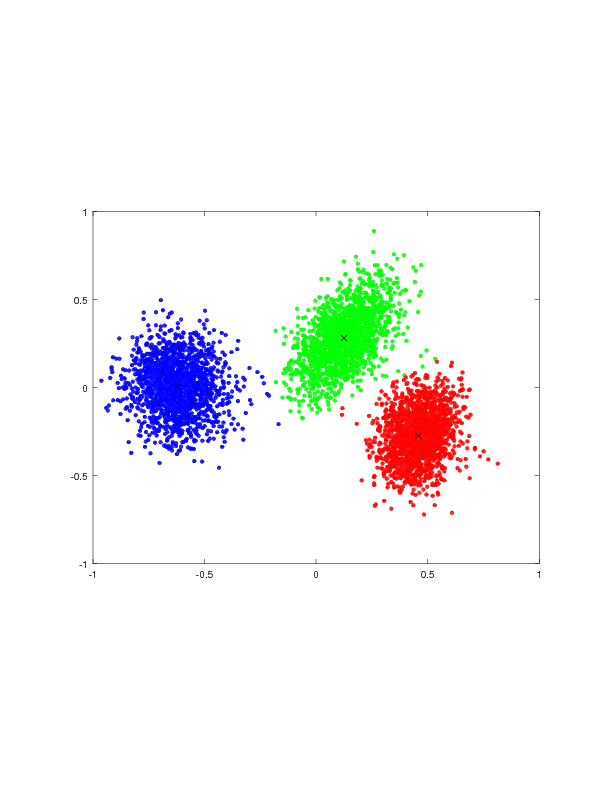
\includegraphics[width=0.5\textwidth]{q4/k3_1.png}
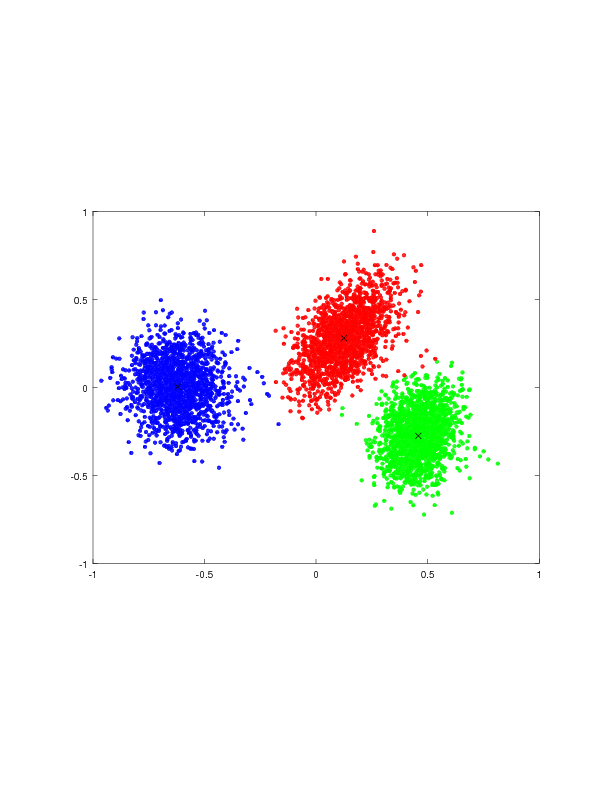
\includegraphics[width=0.5\textwidth]{q4/k3_2.png}
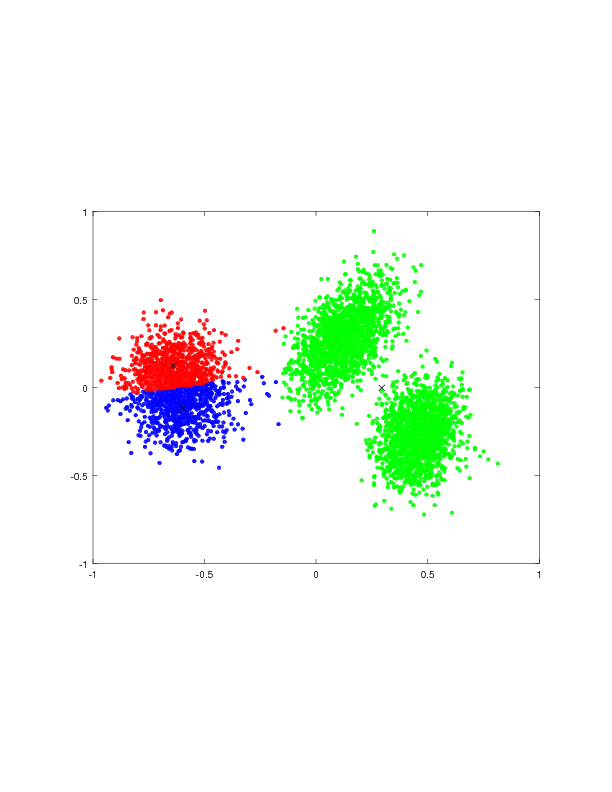
\includegraphics[width=0.5\textwidth]{q4/k3_3.png}
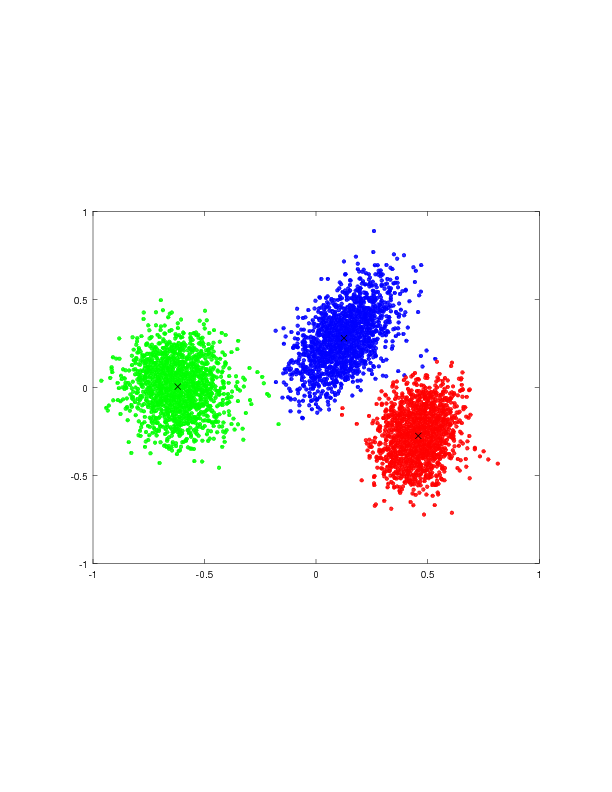
\includegraphics[width=0.5\textwidth]{q4/k3_4.png}

\newpage

\textbf{k = 4}

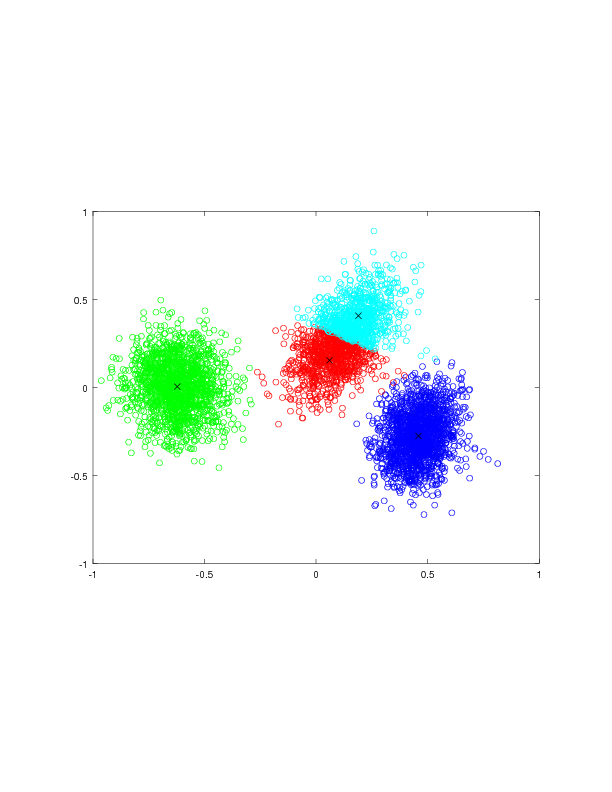
\includegraphics[width=0.5\textwidth]{q4/k4_1.png}
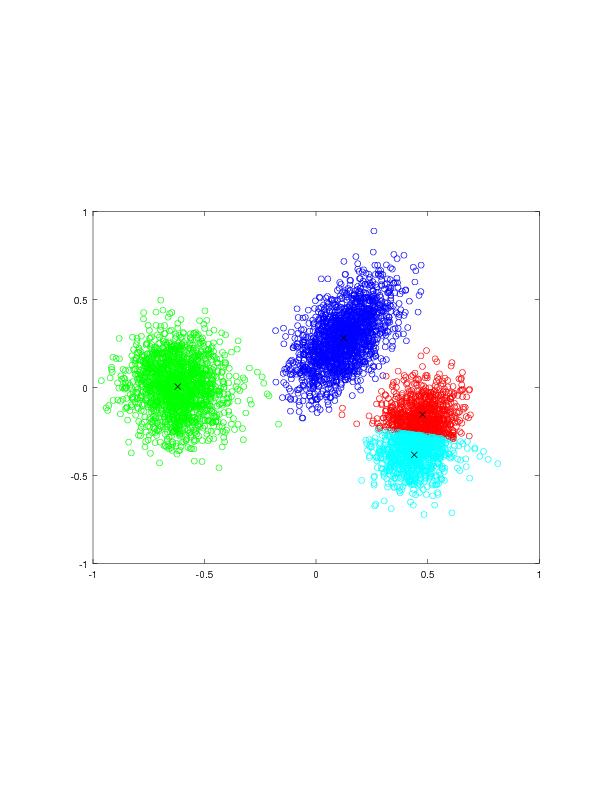
\includegraphics[width=0.5\textwidth]{q4/k4_2.png}
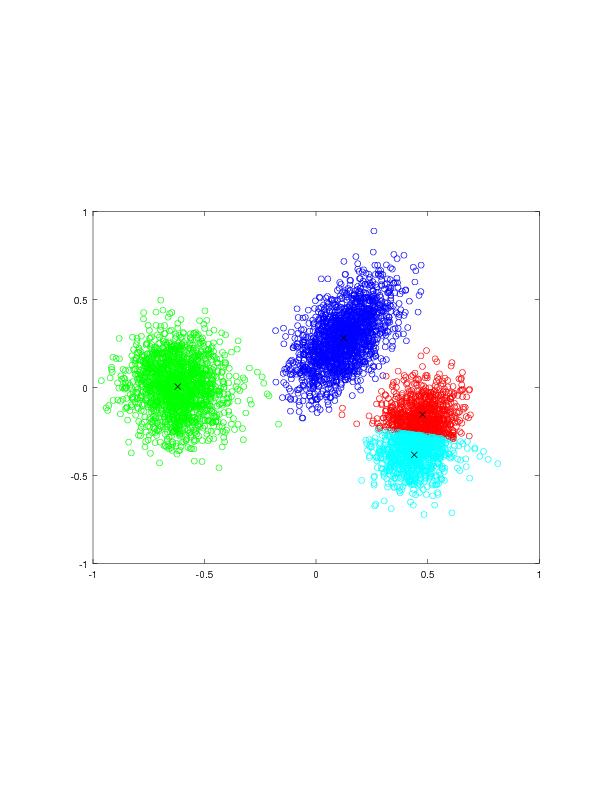
\includegraphics[width=0.5\textwidth]{q4/k4_3.png}
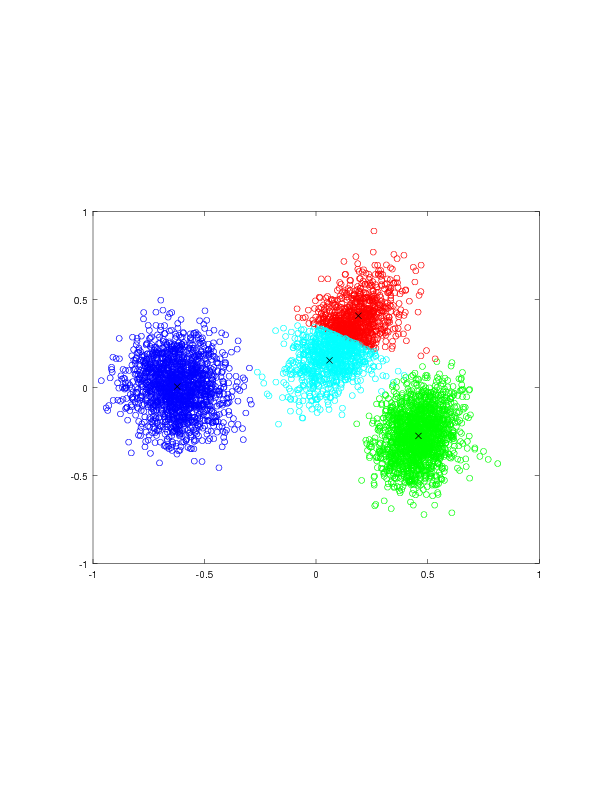
\includegraphics[width=0.5\textwidth]{q4/k4_4.png}

\section*{5}

\subsection*{a)}

Prove that $\ell(\theta^{(t+1)}) \ge \ell(\theta^{(t)})$ \\


Because we chose $Q_i(z^{(i)}) := p(z^{(i)}|x^{(i)};\theta^{(t)})$ in the E-step,\\

$\ell(\theta^{(t)}) = \sum_i \sum_{z^{(i)}} Q_i^{(t)}(z^{(i)}) \log \frac{p(x^{(i)},z^{(i)};\theta^{(t)})}{Q_i^{(t)}(z^{(i)})}$\\

The parameters $\theta^{(t+1)}$ are obtained by the gradient ascent update step\\

$\theta^{(t+1)} = \theta^{(t)} + \alpha \nabla_\theta \sum_i \sum_{z^{(i)}} Q_i^{(t)}(z^{(i)}) \log \frac{p(x^{(i)},z^{(i)};\theta^{(t)})}{Q_i^{(t)}(z^{(i)})}$\\

Because we assume $\alpha$ is small enough to not decrease the objective function, $\theta^{(t+1)}$ will result in a greater than or equal value of the objective function. Using similar logic as in the lecture notes:\\
\begin{align*}
    \ell(\theta^{(t+1)}) &\ge \sum_i \sum_{z^{(i)}} Q_i^{(t)}(z^{(i)}) \log \frac{p(x^{(i)},z^{(i)};\theta^{(t+1)})}{Q_i^{(t)}(z^{(i)})} \quad\text{(by Jensen's inequality)}\\
                         &\ge \sum_i \sum_{z^{(i)}} Q_i^{(t)}(z^{(i)}) \log \frac{p(x^{(i)},z^{(i)};\theta^{(t)})}{Q_i^{(t)}(z^{(i)})} \quad\text{(because of our gradient ascent step as noted above)}\\
                         &= \ell(\theta^{(t)}) \quad\text{(because $Q_i^{(t)}$ was chosen to make Jensen's inequality hold with equality at $\theta^{(t)}$ as noted above)}
\end{align*}
\end{document}
